\section{Connected reductions and coverage through thirteen loops}
\label{sec:notes-loop-tree-results}
The new comparison has three parts. First, 39 requests test connected bubble trees: 34 rational-scale requests cover the distinct star, chain, and branched structures through thirteen loops, and five requests keep the scale symbolic at one, two, three, six, and thirteen loops. Each request contains seven targets: the unit-power integral, three separate positive-power changes, middle-triangle powers zero and minus one, and a simultaneous change of several positive powers. Second, a fresh 110-request grid retains the vacuum, propagator, and scattering definitions of Appendix~\ref{app:families-new} and extends the loop range through thirteen. It includes massive and massless cases, dots, auxiliary numerators, scaleless sectors, and additional symbolic requests. Third, sixteen planar and nonplanar two-loop box batches test the unchanged learned choices at a new kinematic profile.

Every timing starts a fresh process. It includes initialization, domain recognition, model loading and prediction when used, exact reduction, internal checks, recovery, output, and process exit. Independent checks against Gamma expressions or the competing reduction are performed after this application timer. Their cost is benchmark validation overhead and is excluded from both methods. This timer therefore differs from the preceding supplied-basis comparison, which also includes its external reference comparison. We do not combine the two timing totals. Two single-core workers run on shared cluster nodes. Each request compares methods on the same worker, rotates their order, and uses three repetitions for the connected-tree and learned-control tests. The broad coverage grid uses one bounded trial per method. Its completion counts include basis integrals and do not measure how many targets require a nontrivial reduction. The common application limit is twenty seconds; a failed first attempt remains recorded and receives no completed-time ratio.

The development checks compare 42 coefficients exactly with complete symbolic Gamma expressions. Native Kira verifies 5 of the six requests, supplying 35 exact coefficient checks through three loops, including one symbolic-scale request. The remaining three-loop chain reaches the native time limit. The analytic expression passes its symbolic check, and that native timeout remains recorded. Seven tests reject masses, off-shell kinematics, unsupported auxiliary numerators, cuts, symbolic indices, a removed end line, and a cyclic attachment.

For the reserved connected trees, independent complete Gamma evaluations check 819 coefficient values at three dimensions with 80-digit arithmetic. The relative tolerance is $10^{-60}$. These evaluations test the implementation; the identity in Appendix~\ref{app:notes-loop-tree} supplies the analytic justification. They are not independent native IBP reductions at high loop order. All 39 requests, containing 273 target entries, pass these checks and all repeated outputs agree exactly.

\begin{table}[!htbp]\centering\small
\caption{Completion on the fresh requests. The preceding application is the exact-triangle and learned-batch method of Section~\ref{sec:notes-analytic-batch-results}. The broad grid uses one bounded trial. The other collections require three successful repetitions. Failures remain in the denominator.}
\label{tab:notes-loop-tree-completion}
\begin{tabularx}{\linewidth}{@{}Yrrr@{}}\toprule
Collection & Requests & New method & Preceding method\\\midrule
Connected bubble trees & 39 & 39 & 4 \\
Broader physical grid & 110 & 68 & 68 \\
Fresh native box batches & 16 & 16 & 16 \\
\bottomrule\end{tabularx}\end{table}

\begin{table}[!htbp]\centering\small
\caption{Application times on completed, checked pairs. Times are sums of request medians in seconds. The ML-off control keeps the same exact methods and fixed sparse action. The learned-control row measures both retained native learned choices together.}
\label{tab:notes-loop-tree-times}
\begin{tabularx}{\linewidth}{@{}Yrrrr@{}}\toprule
Comparison & Pairs & New & Control & Ratio\\\midrule
Connected trees / preceding & 4 & 0.654 & 4.144 & 0.158 \\
Box batches / preceding & 16 & 51.875 & 52.052 & 0.997 \\
Box batches / ML off & 16 & 51.875 & 55.306 & 0.938 \\
\bottomrule\end{tabularx}\end{table}

The connected-tree application takes between 129.2 and 308.9 milliseconds per seven-target request across the tested orders. On 4 pairs completed by both methods, its summed median is 0.654 seconds against 4.144 seconds, a speed factor of 6.34. The application also returns coefficients for connected requests that the preceding method cannot complete within the declared bounds. Those additional completions have no finite speed factor against a completed control. The matched timings include the exact identity, its one-element basis, and earlier dispatch, so they do not assign every saved second to algebra alone.

On the sixteen fresh native box batches, the retained ML choices use 6.2\% less time than the fixed control. The ratio is 0.938, with request-resampling interval $[0.856,1.021]$. The interval includes equal time, so this small fresh sample does not resolve a reliable added ML gain. The learned method is slower on 9 individual batches. These results remain separate from the preceding forty-request result, where the added batch choice saved 2.7\% against its fixed-action control.

\begin{figure}[!htbp]\centering
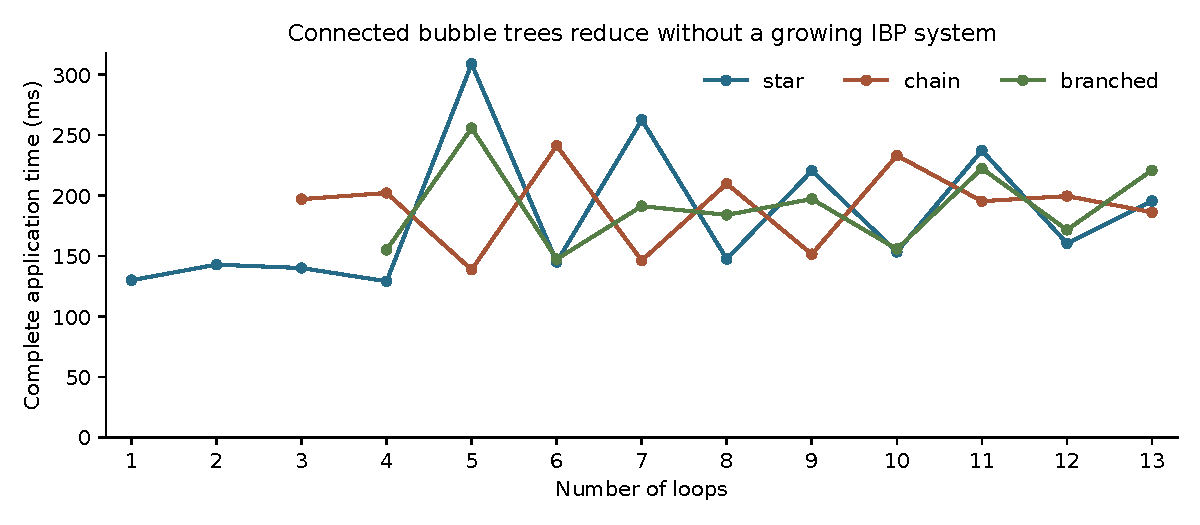
\includegraphics[width=\linewidth]{paper_figures/loop_coverage13_time.pdf}
\caption{The connected bubble-tree formula avoids a growing IBP system. Each point is the median complete application time for seven targets at the indicated loop count. The curves show rational-scale requests; the five symbolic requests enter the completion and check totals. Three repetitions measure process-level variation.}
\label{fig:notes-loop-tree-time}
\end{figure}
\begin{figure}[!htbp]\centering
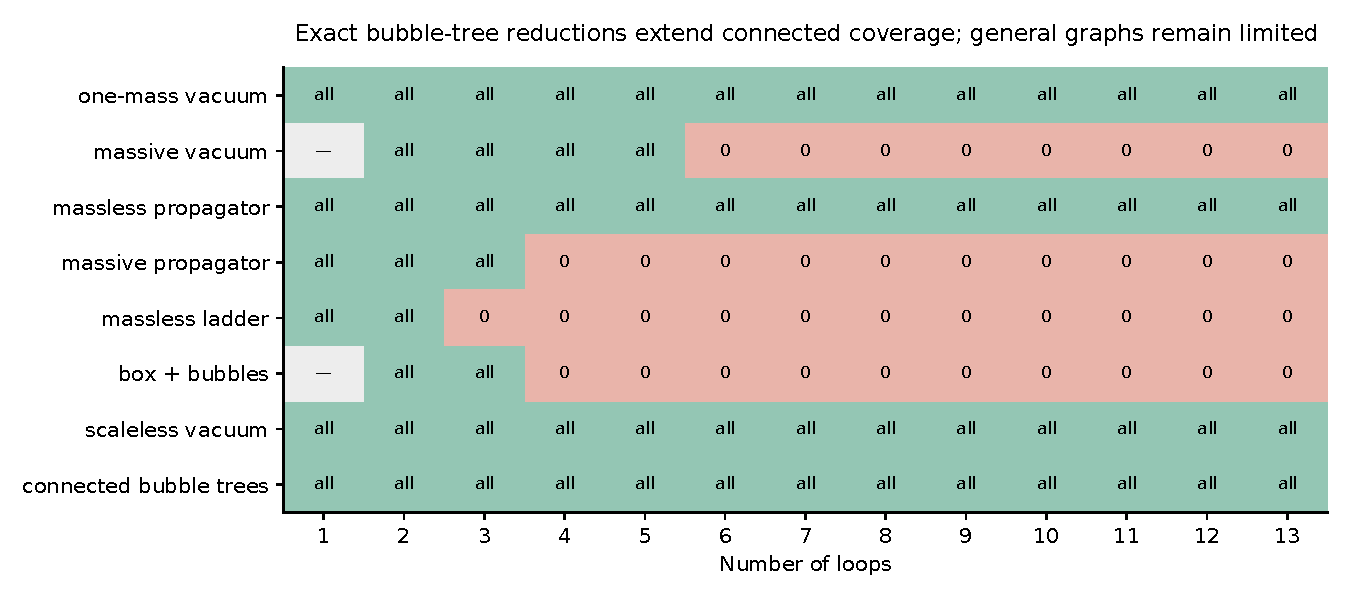
\includegraphics[width=\linewidth]{paper_figures/loop_coverage13.pdf}
\caption{Finite coverage at each loop order. ``All'' means that the method completed every request in that cell, and zero means none completed. A dash marks an omitted duplicate one-loop definition. The connected-tree row includes rational and symbolic requests; the other rows show the main rational grid. Additional scattering and symbolic cases remain included in Table~\ref{tab:notes-loop-tree-completion}. The figure describes these defined targets, not all integrals at that order.}
\label{fig:notes-loop-tree-coverage}
\end{figure}
\begin{table}[!htbp]\centering\small
\caption{Completion by loop order on the full broader grid and the added connected trees. Each entry gives completed requests divided by requested cases for the new method. The preceding-method column applies to the broader grid.}
\label{tab:notes-loop-tree-orders}
\begin{tabular}{@{}rrrr@{}}\toprule
Loops & Broader grid & Preceding grid & Connected trees\\\midrule
1 & 12/12 & 12/12 & 2/2 \\
2 & 12/12 & 12/12 & 2/2 \\
3 & 8/10 & 8/10 & 3/3 \\
4 & 4/7 & 4/7 & 3/3 \\
5 & 4/7 & 4/7 & 3/3 \\
6 & 5/10 & 5/10 & 4/4 \\
7 & 3/7 & 3/7 & 3/3 \\
8 & 3/7 & 3/7 & 3/3 \\
9 & 3/7 & 3/7 & 3/3 \\
10 & 3/7 & 3/7 & 3/3 \\
11 & 3/7 & 3/7 & 3/3 \\
12 & 3/7 & 3/7 & 3/3 \\
13 & 5/10 & 5/10 & 4/4 \\
\bottomrule\end{tabular}\end{table}

The broader grid completes 68 of 110 requests with the new method and 68 with the preceding application. The unresolved cases include general massive multi-loop integrals and multi-scale scattering structures that do not have the proved bubble-tree form. The input limits of the configured native path and application deadlines remain explicit outcomes. A complete scalar-product basis can exceed the index limit of that path even when an analytic subintegral formula remains valid. Thus loop count alone does not determine whether the reduction succeeds. The new result extends a connected analytic domain through thirteen loops; it does not establish acceleration for every integral type.
\FloatBarrier
